%-----------------------------------%
%----- Misc. Document Settings -----% 
%-----------------------------------%
\documentclass[11pt]{article}
\usepackage{preamble}
\usepackage{variables}


%----------------------------%
%----- Title Page Setup -----%
%----------------------------%
\renewcommand*{\thefootnote}{\fnsymbol{footnote}}

\title{\papertitle\footnote{We thank Dan Sunderland, Aizhan Anarkulova, Matt Baugh, Jesse Chan, Zach Kowaleski, Wei Zhou, and workshop participants at Penn State University, the University of Oklahoma, and the University of Texas-Austin Audit Research Reading Group for helpful comments. All the code used to produce this paper is available on GitHub (\url{https://github.com/njhallman/gender-public}). The corresponding author is Nicholas Hallman (\url{nicholashallman@utexas.edu}).}}


\author{
    \vspace{.5cm}Jade Chen\textsuperscript{a}, 
    Nicholas Hallman\textsuperscript{b} and, 
    Jayanthi Sunder\textsuperscript{c}, 
}


\affil{\vspace{.5cm}\textsuperscript{a}Loyola Marymount University}
\affil{\textsuperscript{b}The University of Texas at Austin and the Salem Center for Policy}
\affil{\textsuperscript{c}The University of Arizona}


\date{First Draft: October 2023 \quad $\vert$ \quad Current Draft: April 2025}

\renewcommand*{\thefootnote}{\arabic{footnote}}
\setcounter{footnote}{0}

\begin{document} % <--- Note that the document technically begins here 


%-------------------------------------%
% Response Memos (not in public repo) %  
%-------------------------------------%

% \clearpage
% \input{Response Memos/Response_AE}

% \clearpage
% \input{Response Memos/Response_R1}

% \clearpage
% \input{Response Memos/Response_R2}


%--------------------------%
%-------- Title Page-------%
%--------------------------%
\pagenumbering{gobble}
\maketitle % <--- Insert title page here with the abstract

%------------------------%
%-------- Abstract-------%
%------------------------%
\newpage
\pagenumbering{gobble}


\centerline{\LARGE\papertitle}


\vspace{1cm}
\normalsize


\noindent
\textbf{Abstract:} Both popular media and academic research have long asserted that the Big 4 audit firms (``the firms'') are ``boys clubs'' that fail to equitably retain and promote female auditors. Recently mandated Form-AP disclosures have reignited interest in gender disparities at the firms by revealing that, despite their explicit commitments to gender equity, only a small proportion of their public company engagements are led by female audit partners. We use newly available data on nearly 150 thousand rank-and-file auditors to show that these assertions about gender disparities at the firms were historically accurate. Throughout the 1990s and 2000s, female auditors faced lower retention and promotion rates than their male counterparts. These disparities were even more pronounced in auditing than in most other financial services professions. However, we also show that these disparities narrowed among auditors during the mid-2010s and reversed by the late 2010s. Indeed, we present evidence which suggests that from the late 2010s through the end of our sample period in 2023, it was \textit{male} auditors who were at higher risk of leaving the firms and faced lower probabilities of promotion conditional on staying. The absence of a similar reversal in retention rates for other financial services professions during the same period bolsters our conclusion that the trends observed are not driven by broader industry or labor market factors.

\vspace{5mm}
\noindent
\textbf{Keywords:} gender disparities; auditing; retention and promotion
    
\vspace{5mm}
\noindent
\textbf{Data and Code Availability:} The data used in our analysis was obtained from public sources as described in detail in the paper and in our code. All the code used to produce this paper is available on GitHub. The name of the repository is included on the title page of this manuscript and not on this abstract page to preserve anonymity.

%-----------%
% Main text %
%-----------%
\newpage
\pagenumbering{arabic}
\normalsize
\doublespacing

\section{Introduction} \label{section:Intro}
    The fields of accounting and finance have long been characterized as ``gendered'' professions, marked by significant disparities in career outcomes between men and women \parencite{daltonWomenManagersPartners1997}. These disparities have been noted with concern in the financial press (e.g., \cite{rapoportWomenRarelyRun2018,jaekelWhyWomenArent2016}) and by some of the largest companies in the financial services industry (e.g., \cite{deloitteLeadershipRepresentationGender2022}). The Harvard Business Review claims that ``women's prospects are significantly worse in financial services than in other sectors'' \parencite{jaekelWhyWomenArent2016}. A recent report by McKinsey \& Company discusses a ``leaky pipeline'' from which women are ``falling out in greater numbers as they progress up the career ladder''  \parencite{ellingrudkweilinClosingGenderRace2021}. 
    
    While complaints about a ``boys club'' culture in financial service firms are not new, the recent implementation of Form-AP disclosures has renewed interest in these disparities at the Big 4 audit firms by revealing that only a small proportion of public company audits are led by female audit partners.\footnote{In 2016 the SEC approved a PCAOB proposal requiring audit firms to disclose the identity of the lead audit partner for each public company audit. This disclosure is made on ``Form AP'' and became mandatory for audit reports issued after January 31, 2017. The Big 4 firms are Deloitte, PricewaterhouseCoopers (PwC), Ernst \& Young (EY) and KPMG. Throughout the paper we refer to these firms collectively as ``the Big 4 firms'' or just ``the firms.''} This revelation has generated significant attention in the financial press (e.g., \cite{rapoportWomenRarelyRun2018, lucasWhyFewWomen2025,kissinBigFourAccounting2025}) and seems to contradict the firms' claims that they have made substantial efforts to retain female professionals. The firms point to the implementation of generous family leave opportunities, flexible work schedules, mentorship programs, and female employee resource groups, and they have even tied ``bonuses for partners to targets for female recruitment, promotion, and retention'' \parencite{marriageBigFourAccountants2018}. These efforts, along with the firms' many claims regarding the ``moral and economic imperatives to improve career outcomes women'' have resulted in repeated appearances on lists such as the ``FORTUNE Best Workplaces for Women'' and ``The Times Top 50 Employers for Women.''\footnote{For example, EY says it aims ``to achieve 50\% representation for women... at partner rank by 2025,'' noting that ``if an organization does not leverage the potent weapon of diversity, it risks limiting its creative potential and ultimately losing its competitive edge'' \parencite{eyEYUSDiversity2022, edgleyDiversityProfessionalismBig2016}. PwC claims that ``balanced gender representation across [their] business is a key focus area'' and that the firm is ``focused on supporting equal levels of female representation throughout [their] pipeline'' \parencite{pwcGenderEquity2023}. Deloitte claims that ``gender equality is an important moral initiative,'' that it is ``a vital enabler in companies being successful,'' and that ``inclusive companies are 1.7x more likely to be innovation leaders in their market and businesses with more inclusive and diverse cultures achieve 2.2x higher sales and 3.2x higher profits'' \parencite{davidsonHowEquityCan2023}.}  Yet, despite these programs and attestations (and the resulting accolades), the revelation that so few female auditors are running public company audits has lent credence to claims that the firms remain ``boys clubs'' struggling to shake their sexist pasts \parencite{kellsBigFourAccounting2018}. 
    
    Form-AP disclosures notwithstanding, whether the Big 4 firms have been successful at improving career outcomes for female auditors remains an open empirical question. As the firms themselves have argued, ``boosting the number of female partners takes time, owing to the need to build a pipeline of candidates with sufficient experience to be promoted'' \parencite{kissinBigFourAccounting2025}. Becoming a partner at a Big 4 firm can take 15 years or more. Thus, even effective changes that improve retention and promotion rates for female auditors will take many years to be reflected in Form-AP disclosures. In the meantime, it remains unclear whether we should expect the sorts of policies implemented at the firms to be effective at improving the retention and promotion prospects for the rank-and-file auditors making their way through the firms hierarchies. On the one hand, some research suggests that relatively simple changes, such as updating the numerical scale on which employees' performance is evaluated, can meaningfully improve prospects for women \parencite{riveraScalingInequalityRating2019}. On the other hand, research also suggests that some impediments women face to advancement in the workplace stem from less tractable issues that may be outside the control of the firms, such as societal norms on the division of childcare responsibilities at home \parencite{duLockedinHomeGender2023}. Moreover, interview-based research suggests that some Big 4 firm interventions designed to support female professionals, such as flexible work initiatives, ``actually reinforced gender barriers'' \parencite{kornbergerChangingGenderDomination2010}.
    
    In this paper, we examine the firms' progress towards their stated goal of gender equity. Our analysis uses newly available data on the careers of nearly 150 thousand unique Big 4 auditors of all levels and spanning several decades.\footnote{See \url{https://www.reveliolabs.com}.} We track these auditors from the outset of their careers—typically right out of college—and as they advance through the ranks of (or exit) the firms. To provide a point of reference, we also track the careers of nearly 2.4 million professionals in other financial service roles (e.g., investment bankers, actuaries, credit analysts, etc.). These data allow us to compare the retention and promotion rates of men and women, both within and outside the auditing professions, and track the differences and changes over a long time series.
           
    Consistent with claims that ``women are far more likely than men to leave the [financial services] industry'' and that ``men are promoted at materially higher rates than women'' \parencite{jaekelWhyWomenArent2016}, our findings reveal that, historically, female auditors experienced a significantly lower retention rate than their male colleagues. This disparity was even larger in auditing than in other comparable financial services. However, unlike in other financial services, the gender disparity in auditing began to subside in the mid 2010s. By the late 2010s, and through the end of our sample period in 2023, female auditors were retained at \textit{higher} rates than their male counterparts. This finding is robust to controls for the race and educational attainment of auditors, as well as fixed effects for audit firms, calendar year, starting cohort, and metropolitan statistical area. Our findings are similar when we use hazard models instead of ordinary least squares. We also show that gender disparities in promotion rates have followed a similar trajectory, reversing from a female promotion \textit{disadvantage} as late as 2011 to a female promotion \textit{advantage} in 2016 and later. While the focus of this study is on relative rates of retention and promotion between male and female auditors, it is noteworthy that the retention rate for both men and women has increased during the later half of our sample relative to the early years.

    Many factors likely contributed to the increase in the retention of female auditors that we document. However, one policy implemented during our sample period attracted particular attention: equalized family leave programs (i.e., providing male and female employees the same amount of paid time off after the birth or adoption of a child). We leverage the staggered implementation of these policies at three of the four Big 4 firms to show that they partially explain the relative improvement in the retention of female auditors. Interestingly, however, this relative improvement is driven by a \textit{decrease} in the retention of male auditors at firms that implemented equalized leave, not by an \textit{increase} in the retention of female auditors. This evidence differs from that found by recent work in other settings such as academia \parencite{antecolEqualInequitableWho2018} and suggests that the effects of equalized family leave policies are likely context-dependent. 
    
    Our findings stand in contrast with recent academic research and articles in the popular press which show that women are underrepresented among Big 4 audit partners \parencite{burkeAuditPartnerIdentification2019, leeAuditPartnerAssignments2019, rapoportWomenRarelyRun2018}, and which claim that the Big 4 accounting firms ``struggle to retain women'' \parencite{kornbergerChangingGenderDomination2010}. This seeming contradiction is likely a matter of timing. We show that there was a large increase in the relative retention and promotion rates of female auditors in the 2010s, and yet most attempts to assess the state of gender equity in the auditing industry either predate these changes \parencite{kornbergerChangingGenderDomination2010, daltonWomenManagersPartners1997,anderson-goughHelpingThemForget2005} or focus exclusively on audit \textit{partners} \parencite{burkeAuditPartnerIdentification2019, leeAuditPartnerAssignments2019, rapoportWomenRarelyRun2018}. Because it typically takes many years for a newly hired auditor to reach the rank of partner, and longer still for them to lead the audits of the largest and most visible public clients, the auditors that are the focus of recent attempts to measure gender equity in the profession began their careers in the 1990s and 2000s. Our findings suggest that real changes have been made within the accounting firms long after many current partners entered the profession, and that these changes have had significant effects on the retention and promotion of the female auditors who are currently making their way through the Big 4 talent pipeline. 

    Our findings are consistent with, and complementary to, contemporaneous research by \textcite{ahnDiversityCareerTrajectories}, who also use Revelio data to study disparities in turnover and career outcomes between male and female auditors (among other demographic groups). They focus on estimating average differences in retention and career outcomes over their sample period (2008-2021), and on identifying cross-sectional factors (e.g., same-group representation) that affect retention and promotion rates of ``diverse'' auditors. By contrast, we document \textit{changes} in the relative prospects of male and female auditors over time. This is an important difference, as the sample period used by \textcite{ahnDiversityCareerTrajectories} is centered on the major shift in the relative retention of female auditors that we document in the mid-2010s. \textcite{ahnDiversityCareerTrajectories} also study the auditing profession in isolation, whereas we benchmark the changes we document in auditing against other financial service professions.
    
    Finally, our findings have significant implications for broader economic and institutional dynamics. First, the demographic composition of Big 4 audit practices has substantial spillover effects into corporate leadership structures. Nearly 20 percent of public companies have at least one c-suite executive who formally served as an audit manager or partner at a large public accounting firm, and more than 75 percent have at least one such person on their board \parencite{albrechtAuditorsRecognizePotential2018}. Thus, changes in the gender composition of audit leadership are likely to propagate through corporate governance channels. Second, given that the Big 4 firms employ tens of thousands of professionals and oversee financial reporting for more than 99 percent of S\&P 500 companies \parencite{pakalukAuditorMarketShare2017}, their institutional practices have outsized influence on market integrity and professional development in financial services. Third, our findings provide empirical validation of institutional interventions aimed at gender equity. While anecdotal evidence has suggested that the Big 4 firms pursue gender equity more aggressively than other financial services institutions, we document that these efforts have yielded measurable outcomes - specifically, a reversal of historical disparities resulting in statistically significant retention and promotion \textit{advantages} for female auditors over their male colleagues in recent years. Furthermore, our analysis of equalized family leave policies, which the Big 4 firms pioneered in the United States \parencite{ballesteroImportanceOrganizationalCulture2023}, provides initial evidence on the effectiveness of a specific institutional intervention. These findings create opportunities for future research examining the precise mechanisms through which organizational policies influence gender-based retention dynamics in professional service firms.

\section{Sample design and coverage} \label{section:Data}  
    
    \subsection{Sample design} \label{section:sampleDesign}
        We obtain data on the careers of auditors and professionals in other financial services (OFS) from Revelio. Revelio collects and standardizes data from ``hundreds of millions of public employment records'' and provides access to ``current and historical workforce composition and trends of any company.''\footnote{Revelio claims to collect data from ``a variety of publicly accessible online data sources, including online professional profiles, online employee reviews, job postings from company career pages and aggregator sites, and WARN layoff notices.'' See \url{https://www.data-dictionary.reveliolabs.com}.} As noted by \textcite{agrawalInformationDispersionEmployees2021}, a large proportion of the U.S. workforce creates profiles on platforms such as LinkedIn (a primary data source for Revelio), particularly in the industries of finance and business services. 
        
        We create our sample by querying Revelio via WRDS for all records related to auditing and comparable roles in OFS. Our query starts with Revelio's \textit{individual\_positions} table, which tracks employee-employer relationships.\footnote{A single employee can have multiple positions at the same firm over time. For example, an auditor may be promoted from staff to senior, and then to manager. Revelio will record each of these ranks as separate positions, with separate start and end dates, so long as the auditor records their promotions in their online profile in a way that is interpretable by algorithms Revelio uses to standardize the data.} We retrieve all records in the \textit{individual\_positions} table with values of \textit{role\_k1500} that match one of those listed in the Appendix (see Table \ref{table:rolesTable}).\footnote{We reviewed a list of all unique values of the \textit{role\_k1500} variable in the \textit{individual\_positions} table and, in addition to roles related to auditing, we used our best judgment to select a set of financial service roles that would make for a meaningful comparison to auditing. All the code that we used to query Revelio and perform our analysis is available in a convenient replication package on GitHub. We encourage interested readers to explore the effects of different samples and design choices.} We also retrieve fields from the \textit{individual\_positions\_raw}, \textit{individual\_user}, \textit{individual\_user\_raw}, and \textit{individual\_user\_education} files for each user and position that matches our initial query.
        
        To create our auditor sample, we limit the data retrieved from the Revelio query to positions for which \textit{role\_k1500} is equal to either ``audit'' or ``auditor'' and for which \textit{company\_raw} is equal to a common variant of the name of one of the Big 4 accounting firms.\footnote{We specifically screen for the following values of \textit{company\_raw}: pwc, pricewaterhousecoopers, pricewaterhousecoopers llp, price waterhouse coopers, pricewaterhousecoopers, llp, ey, ernst \& young, ernst \& young llp, ernst \& young, llp, ernst and young, e \& y, deloitte, deloitte \& touche, deloitte \& touche llp, deloitte \& touche, llp, deloitte and touche, kpmg us, kpmg, kpmg llp, kpmg, llp, kpmg audit. We arrived at this set of values by sorting the unique values of \textit{company\_raw} in the \textit{individual\_positions} table by number of unique employees and reviewing those associated with a significant number of employees to determine if they represent a variant of the name of a Big 4 accounting firm.\label{footnote:firmNames}} This process results in a sample of 192,245 unique Big 4 auditors associated with 292,897 unique positions. For purposes of our analyses, we drop positions with missing start dates or with start dates that fall after their end dates. We also drop auditors that move between the Big 4 firms during our sample period, auditors missing educational data, and internship positions.\footnote{Our results are not sensitive to including auditors that change audit firms or to including auditors with missing educational data and removing educational attainment controls from our model.} We then use the start and end dates of each remaining position to create a panel of 766,730 auditor-year observations. After dropping 2024 to ensure we can measure retention and promotion outcomes for one year following the end of our sample period, we are left with our primary sample - a panel of 713,614 auditor-year observations associated with 145,573 unique auditors.
        
        For each auditor-year observation, we attempt to assign a rank of either staff, senior, manager, senior manager, director, or partner based on the value in the \textit{title\_raw} field. However, many auditors' historical titles appear to be overwritten in the Revelio data when they are promoted, making the assignment of their historical ranks impossible. For example, some senior auditors only have one position-level record in the Revelio dataset. Often the start date of this position appears to be the beginning of the auditors' career at the firm, not the date of their promotion to senior.\footnote{For example, taken at face value the Revelio data suggests that some auditors entered their firms directly out of college at the rank of senior and held that rank for six years before leaving. Such observations are suspect for two reasons. First, Big 4 auditors normally only hold the rank of senior for between 3 and 4 years. Second, the Big 4 firms hire almost exclusively out of universities and to fill staff-level positions. For a small sample of auditors that appear to enter the sample at a rank higher than staff, we manually visited their LinkedIn profiles and found that some only disclose their final rank at their firm while others disclose prior ranks in non-standard ways (e.g., in the text of their profile description) that are likely missed by the algorithm that Revelio uses to clean their data.} For our promotion analysis, we drop auditors for whom we are unable to infer historical ranks from the sample, leaving a panel of 284,999 auditor-year observations. The sample selection process is summarized in Table \ref{table:sampleDesign}. The composition of the primary sample by gender and rank is shown in Figure \ref{figure:stackPlot}.
        
        To create our sample of OFS professionals, we limit the data retrieved from the Revelio query to positions for which \textit{role\_k1500} is equal to any of the values in Table \ref{table:rolesTable} \textit{except} for ``audit'' or ``auditor'' and for which \textit{company\_raw} is \textit{not} equal to a common variant of the name of one of the Big 4 firms (see footnote \ref{footnote:firmNames}). We drop positions with invalid or missing start dates or with start dates that fall after their end dates. We also drop ``self-employed'' positions, positions at companies without valid names or IDs, and positions at H\&R Block, which primarily employs preparers of simple personal tax returns that we do not consider a good comparison group for Big 4 auditors. We drop employees who are missing educational data and those who  do not have at least a bachelor's degree. Finally, we drop internship positions. We then use the start and end dates of each remaining position to create a panel of 23,334,598 financial service professional-year observations. After dropping 2024 to ensure we can measure retention outcomes for one year following the end of our sample period, we are left with a sample of 21,126,043 financial service professional-year observations associated with 2,397,919 unique financial service professionals. The sample selection process is summarized in Table \ref{table:sampleDesign}. A list of the top 50 companies employing the OFS professionals in this sample is provided in the Appendix (see table \ref{table:employerTable}).

    \subsection{Sample coverage}\label{section:sampleCoverage}
        The Big 4 accounting firms do not systematically disclose headcount statistics for their audit practices. However, one-off disclosures suggest that our sample covers a large majority of Big 4 auditors, at least in the later years of our sample period. For example, KPMG discloses employing 8,645 auditors in the United States in 2019 \parencite{kpmg2022ApproachAudit2022}. Our primary sample, after the data screens described in Table \ref{table:sampleDesign}, contains 8,107 of those auditors. An important caveat is that the number of auditors we observe drops significantly for earlier years, as demonstrated by Figure \ref{figure:stackPlot}. There are three likely reasons for this drop. First, the Big 4 accounting firms have increased their headcount over time, so we would expect to observe more auditors in later years even if our sample captured the entire universe of Big 4 auditors. Second, the public accounting industry used to be dominated by the ``Big 8'' firms until a series of mergers and acquisitions in the 1980s and 90s (along with the demise of Author Andersen in 2002) produced the modern Big 4. We only capture auditor-years that are associated with Big 4 firms. Third, LinkedIn started in 2003. Any auditor who dropped out of the workforce before 2003 is unlikely to appear in our sample.\footnote{Although we cannot track auditors who left the workforce prior to creating a LinkedIn profile, we \textit{can} and do trace former auditors who eventually post resumes back to their start and exit dates at the firms, even if they did not create an online profile until after they left public accounting. For example, an auditor who started their career as an auditor in 1995 would enter our panel in that year, even if they left for a corporate accounting role in 2000 and did not create an online profile until 2012. Thus, our panel includes many auditor-years that predate the existence of LinkedIn.} 
        
        This third reason could confound our attempts to compare male and female retention rates over time. We only observe work histories for individuals who eventually post their resumes online. Auditors who permanently exit the workforce prior to the popularity of LinkedIn likely never create professional online profiles and are systematically excluded from our sample. Because women have historically been more likely to leave the workforce than men \parencite{blauFemaleLaborSupply2013}, we acknowledge that, early in our sample period, we are likely to underestimate the proportion of auditors who are female. Moreover, if the female auditors excluded from our early sample had shorter careers in the Big 4 firms than the female auditors that do make it into our sample (which seems likely as, holding start dates constant, women with longer careers are more likely to still be working when LinkedIn came online and became ubiquitous), we will overestimate the female retention rate early in the sample period. We expect this bias to reverse later in the sample period, as it becomes less likely that workers will leave the workforce before posting their resume to professional networking sites, regardless of career length. Overestimating female retention early in our sample period works against our ability to find an improvement in female retention rates over time, and our results should be interpreted with this caveat in mind. As discussed in more detail in the following sections, we also attempt to mitigate this concern by benchmarking any changes in retention rates that we find in auditing against OFS professions, which are likely to be affected by the same bias. 
    
\section{Analysis}\label{section:analysis} 

    \subsection{Primary model}\label{section:byperiod}
        Much of the conventional wisdom about gender disparities in retention and promotion rates in accounting firms comes either from survey evidence \parencite{kornbergerChangingGenderDomination2010,daltonWomenManagersPartners1997, anderson-goughHelpingThemForget2005} or from examining the gender composition of partners who sign public company opinions and therefore appear in Form AP disclosures \parencite{rapoportWomenRarelyRun2018, burkeAuditPartnerIdentification2019}. One issue with this prior work is that it usually captures a single point in time, making it impossible to examine changes \textit{over} long periods of time. Moreover, most surveys predate contemporary campaigns for equity in the workplace and explicit commitments by the Big 4 audit firms to improve female representation. Even the more recent work studying Form AP data effectively examines the outcomes of human resource decisions made decades ago, as such work can only observe audit \textit{partners} who typically started their careers in the late 1990s or early 2000s. In light of these limitations, we begin our analysis by examining how gender differences in retention for rank-and-file auditors at the Big 4 accounting firms have changed over time. 

        To accomplish this task, we create indicator variables representing each two-year period from 2010 through 2019. We also create an indicator variable representing all years prior to 2010, and another representing all years after 2019. We then interact these period indicators with an indicator variable for female auditors (\FEMALE) and fit the following linear probability (LPM) model: 

        \vspace{-6ex}
        \begin{align}\label{eq:primaryModel}
            \textit{ Prob.}(&\RETAINED_{i,t+1})= \gamma_0+\gamma_1*\FEMALExPREX_{i,t} + \gamma_2*\FEMALExXtoXI{i,t}+ \\ 
                            &\gamma_3*\FEMALExXIItoXIII{i,t} + \gamma_4*\FEMALExXIVtoXV{i,t} + \gamma_5*\FEMALExXVItoXVII{i,t} + \nonumber\\
                            &\gamma_6*\FEMALExXVIIItoXIX{i,t} + \gamma_6*\FEMALExPOSTXIX{i,t} + \gamma_k*\textit{Controls}_{i,t} + FE + \epsilon_{i,t}\nonumber
        \end{align}

        The dependent variable in \ref{eq:primaryModel} is \RETAINED, an indicator variable which captures whether auditor \textit{i} remains with their Big 4 audit firm the following year. The coefficients $\gamma_1$ through $\gamma_6$ capture the probability of retaining female auditors in each period, relative to the probability of retaining male auditors. The pattern of these coefficients will allow us to determine whether female auditors are at a retention disadvantage as the conventional wisdom suggests, and whether this disadvantage has changed over time.

        \textit{Controls} is a vector of variables that we include in \ref{eq:primaryModel} to help focus our analysis. For example, we control for whether the auditors in our sample have earned master's degrees (\MASTERS) and whether they attended a top university (\TOPUNIV) as defined by \textcite{FGH2022}. We also control for auditors inferred race with three indicator variables (\BLACKRACE, \APIRACE, and \OTHERRACE) which indicate that Revelio has classified the auditor as Black, Asian/Pacific Islander, or another non-White race (e.g., Hispanic) respectively. In addition to these variables, we absorb several sets of fixed effects (i.e., \textit{FE}) in our estimation of \ref{eq:primaryModel}, including (1) starting-year (i.e., cohort-year), (2) calendar-year, and (3) audit-firm.\footnote{As discussed in later sections, we also test the robustness of our findings to the inclusion of fixed effects capturing metropolitan statistical area by calendar year, which we only have for a subset of our sample.} Definitions for all variables are provided in the Appendix (see Table \ref{appendix:variableDefinitions}).

    \subsection{Descriptive statistics}\label{section:descriptiveStatistics}
        Descriptive statistics for both the auditor sample and the sample of OFS professionals are provided in Table \ref{table:summaryStats}. In both samples, relative to men, retention rates are slightly higher for men than for women. Retention rates for both genders are lower for auditors than for OFS professionals (p<0.01, not tabulated). In both samples, women are more likely to be non-white and less likely to have a master's degree. In the auditing sample, there is no significant difference in promotion rates between men and women.\footnote{We do not attempt to track promotions in the OFS sample because rank titles are not as standardized as in the Big 4 firms, making the assignment of comparable ranks across firms very difficult.} All of these differences are based on averages over a very long sample period. In the following sections, we examine how these differences have changed over time.

    \subsection{Primary results}\label{section:primaryResults}
        We present the results of estimating \ref{eq:primaryModel} in Column 1 of Table \ref{table:interactionModels}. The coefficient for \FEMALExPREX\ is negative (-0.012) and significant (p<0.01), indicating female auditors were historically approximately 1.2 percentage points less likely to remain with the Big 4 firms each year. This result is consistent with prior research and conventional wisdom, as discussed in Section \ref{section:Intro}. The coefficients for \FEMALExXtoXI\ and \FEMALExXIItoXIII\ are also negative (-0.022 and -0.011) and significant (both p<0.01), indicating that the retention disadvantage for female auditors persisted into the first half of the 2010s. However, the small (-0.002) and insignificant coefficient for \FEMALExXIVtoXV\ suggests that female auditors were no longer less likely to be retained than their male colleagues by the middle of the 2010s. The coefficients for \FEMALExXVItoXVII, \FEMALExXVIIItoXIX, and \FEMALExPOSTXIX\ are all positive (0.010, 0.011, 0.009) and significant (all p<0.01), indicating that by the latter half of the 2010s female auditors enjoyed a retention \textit{advantage} comparable in magnitude to the disadvantage they faced in previous decades. 

        It is possible that the apparent increase in the retention of female auditors has nothing to do with policy changes at the Big 4 firms, but is driven instead by either a general shift in employment patterns in financial services or by a bias in the way our data are generated and collected (i.e., shifting patterns in the relative propensities of men and women to post their work histories on professional networking sites). We evaluate these alternative explanations by fitting \ref{eq:primaryModel} in our sample of OFS professionals.\footnote{When estimating \ref{eq:primaryModel} in our sample of OFS professionals we replace audit firm fixed effects with employer fixed effects. In the tables, we refer to these both simply as ``employer fixed effects.''} The results are presented in Column 2 of Table \ref{table:interactionModels}, and show that there was a relatively small but remarkably consistent and statistically significant (p<0.01) retention disadvantage for female workers in OFS throughout our sample period. There is no evidence of a change in this pattern over time. 
        
        We provide a visual representation of the patterns revealed in Columns 1 and 2 of Table \ref{table:interactionModels} in Figure \ref{figure:coeffPlot}. Rather than plotting only those coefficient estimates in the table, we take advantage of the figure to provide coefficient estimates over a longer period of time by supplementing \ref{eq:primaryModel} with additional indicator variables (interacted with \FEMALE) for each two-year period going back to 1990 and extending through the end of our sample period in 2023. We then re-estimate the model using both our sample of auditors and our sample of OFS professionals and plot the coefficient estimates. The figure demonstrates that the shift that we document for auditors in the mid-2010s represents a sharp break with a long-standing historical trend. Female auditors were retained at lower rates than male auditors consistently from 1990 through 2013, and this disparity was larger in auditing than in OFS in every period during that time (although the difference is not always statistically significant). Indeed, the retention disadvantage for women was increasing as recently as the late 2000s. Then, quite suddenly, that disadvantage decreased to its lowest level to date in 2014-2015, followed by a pattern of persistent retention \textit{advantage} for female auditors through the end of our sample period in 2023. Meanwhile, the pattern for OFS professionals is much more stable, with a small but persistent retention disadvantage throughout the extended period from 1990 through 2023.\footnote{The one exception is during the financial crisis in the 2008-2009 period, when there was no significant difference in retention between male and female professionals in OFS.}

        Because our OFS sample includes many heterogeneous types of professionals, we perform a similar analysis for two specific financial service roles: investment bankers and credit analysts. The results are presented in Columns 3 and 4 of Table \ref{table:interactionModels}. We find a retention disadvantage for female investment bankers and a retention advantage for female credit analysts. Importantly, both differences are persistent during the mid-2010s, when we document a large improvement in the retention of female auditors.\footnote{We also examined many other roles and found similarly stable patterns in retention disparities in all of them. We chose to tabulate one case where we observed a retention advantage for males and one where we observed a retention advantage for females.} The stable retention rates for female (relative to male) professionals in OFS demonstrate that the improvement in the retention of female auditors at the Big 4 firms is not a general trend in the financial services labor market. They also show that our findings for auditors are not driven by a bias in the way our data are generated and collected, as any such bias would likely affect all financial service roles. 

    \subsection{Additional analysis}\label{section:robustnessTests}

        \subsubsection{Survival analysis}\label{section:survivalAnalysis}
            Our primary analysis relies on an LPM to estimate gender differences in auditor retention, which has the advantage of being familiar and easily interpretable. Next, we estimate a hazard model as an important robustness test. Hazard models explicitly estimate the time until exit, making them well-suited for detecting gender-based differences the timing of auditors' exit from the Big 4 firms over their careers. Hazard models are especially useful when the risk of exit is non-linear over the period of risk exposure, which is likely the case in our setting. That is, gender disparities in retention may manifest not only in differences in overall retention rates each year, but in differences that vary over the course of auditors' careers (e.g., retention rates may be similar for male and female staff auditors but different for male and female seniors). While the inclusion of cohort-year fixed effects in our LPM helps address this issue to some extent, hazard analysis provides a more rigorous approach. 

            We estimate a Cox proportional hazards (CPH) model \parencite{coxRegressionModelsLifeTables1972,statacorpStcoxCoxProportional2023} with the same interactions between \FEMALE\ and calendar-time indicator variables as in \ref{eq:primaryModel}.\footnote{We do not include cohort-year fixed effects in the CPH model because the model itself accounts for length of service, which is perfectly predicted by a combination of cohort-year and calendar-year.} The results are presented in Column 1 of Table \ref{table:robustnessModels}. The log hazard ratio (i.e., the Cox coefficient) for \FEMALExPREX\ is 0.062, which is statistically significant (p<0.01). Exponentiating this coefficient (i.e., $e^{0.062}$) gives the estimated hazard ratio of 1.064 and indicates that, prior to 2010, female auditors were 6.4 percent more likely to exit the Big 4 firms than their male counterparts. For purposes of comparison, the unconditional retention rate of male auditors during this period was 84.4 percent (untabulated), so a rough estimate of the retention rate of female auditors during the same period is $0.844^{1.064} =$ 83.5 percent, a difference of 0.9 percentage points. This is comparable to the 1.2 percentage point retention disadvantage for female auditors during the pre-2010 period estimated in our LPM analysis from Column 1 of Table \ref{table:interactionModels}. 
            
            While the magnitude of the early-sample retention disparity is similar between our CPH model and our LPM, the CPH model suggests a slightly earlier reversal of that disparity. Specifically, the log hazard ratio for \FEMALExXIItoXIII\ is small (0.007) and statistically insignificant (p>0.10), and the log hazard ratio for \FEMALExXIVtoXV\ is negative and statistically significant (p<0.01), indicating that female auditors were at \textit{lower} risk of exiting the firms than their male colleagues during those years. By 2016-2017, the log odds ratios stabilize at around -0.095 and persist at that level through the end of the sample period, suggesting that from the mid-2010s onward, female auditors were approximately nine percent (i.e., $1-e^{-0.095}$) less likely to leave the Big 4 than their male colleagues. 

            In Figure \ref{figure:survivalCurves}, we complement our CPH analysis by presenting Kaplan-Meier survival curves \parencite{kaplanNonparametricEstimationIncomplete1958} estimated separately for male (in blue) and female (in green) auditors in the pre-2012 (solid lines) and 2012-2023 (dashed lines) periods.\footnote{We partition the sample at 2012 because the 2012-2013 period is the first in which we no longer observe female auditors at higher risk than male auditors of exiting the firms in our CPH analysis. Partitioning the sample using 2012 also provides us with enough years to plot 10-year survival curves both pre- and post-partitions.} Like CPH models, Kaplan-Meier estimators help account for right censoring in the data and also allow hazard rates to vary over the course of auditors' careers. 
            
            Figure \ref{figure:survivalCurves} suggests that attrition rates are highest in years 2 through 5 (which is when auditors typically hold the rank of senior and take on significant new responsibilities) regardless of gender or time period. All auditors exhibit substantially higher retention rates in more recent years. For example, the 10-year survival probability for male auditors more than doubled from approximately 12 percent prior to 2012 to approximately 27 percent during years 2012-2023. Consistent with our findings in Column 1 of Tables \ref{table:interactionModels} and \ref{table:robustnessModels}, prior to 2012, female auditors were at a retention disadvantage. The survival curves reveal that the disadvantage started in female auditors third year and persisted through year ten. However, female auditors enjoyed an even larger absolute increase in retention than male auditors, such that female auditors' survival probabilities dominate those of male auditors each year of their careers during the 2012-2023 period. For example, the 10-year survival probability for female auditors nearly tripled, from approximately 10 percent prior to 2012 to nearly 30 percent during the years 2012-2023. This is an important finding, as it suggests that the increase in the retention of female auditors that we document is significant both in relative and in absolute terms, and not driven by a decrease in the retention of male auditors
        
        \subsubsection{Controlling for auditors' geographic location}\label{section:locationControls}
            Next we estimate \ref{eq:primaryModel} using an LPM after replacing calendar-year fixed effects with calendar-year by metropolitan area fixed effects. While missing data reduces the sample for this test by about 20 thousand observations, the more rigorous fixed effects structure allows us to control for city-year variation in conditions such as unemployment, labor force participation, fertility, immigration, etc. The results are presented in Column 2 of Table \ref{table:robustnessModels} and show that our estimates for the coefficients of interest are remarkably stable despite the change in sample and the addition of hundreds of new fixed effects. 

        \subsubsection{Modeling promotion}\label{section:promotionModel}
            Thus far we have limited our analysis to retention outcomes, in part because (as discussed in Section \ref{section:sampleDesign}) we are unable to reliably determine historical ranks for the majority of the auditors in the Revelio data. However, in our next test, we limit our sample to those auditors for whom we can reliably infer historical ranks and model promotion outcomes. To this end, we modify \ref{eq:primaryModel} by changing the dependent variable to \PROMOTED, an indicator variable that captures whether auditor \textit{i} is promoted to a higher rank in the following year. We drop observations at the rank of partner as that rank is typically terminal at the Big 4 firms. We also drop observations for which \RETAINED\ = 0 so that our analysis models promotion \textit{conditional on retention}, distinguishing it from our retention analysis despite the mechanical relationship between retention and promotion in the full sample.  
            
            The results are presented in Table \ref{table:promotionModels} and show that promotion disparities followed a similar pattern to retention disparities. Namely, conditional on remaining at their firms, female auditors were less likely than their male colleagues to be promoted early in our sample period (the coefficients for \FEMALExPREX\ and \FEMALExXtoXI\ are both negative and statistically significant). This disparity disappears in the mid-2010s (the coefficients for \FEMALExXIItoXIII\, \FEMALExXIVtoXV\ and \FEMALExXVItoXVII\ are all statistically insignificant) and reverses in the late 2010s (the coefficients for \FEMALExXVIIItoXIX\ and \FEMALExPOSTXIX\ are both positive and statistically significant).
            
            
        \subsubsection{Equalized family leave}\label{section:equalizedLeave}
            The Big 4 firms implemented many programs and policies designed to improve the retention and promotion of female employees during our sample period, and many such programs likely contributed to the trends we document in previous sections. However, one program - equalized family leave - has attracted significant attention \parencite{ballesteroImportanceOrganizationalCulture2023, picchiPaternityLeaveIgnored2020, connleyHowUnequalPaid2020}. 
                
            The Big 4 firms have long offered new mothers significant amounts of paid time off and flexible work arrangements after childbirth. However, recent studies indicate that auditors working for major accounting firms are hesitant to use such work-life balance benefits for fear that taking advantage of them might lead to adverse long-term career consequences \parencite{buchheitContemporaryAnalysisAccounting2016}. This is perhaps especially true when the benefits are exclusive for female employees, because women may feel they risk falling behind their male colleagues who do not (indeed, historically were not permitted to) take similar amounts of paid time off after the birth of a child. \textcite{kornbergerChangingGenderDomination2010} suggest programs that focus on providing benefits and flexibility to female employees can actually deepen gender barriers because they provide firm leaders ``with an institutionally sanctioned and externally awarded program that demonstrates [their] good intentions and values'' while also allowing them to rationalize ``the lack of progress of women who opted to participate in the program.'' Consistent with these arguments, large-scale research examining female-specific maternal leave programs suggests they may actually \textit{decrease} long-run labor force participation for women \parencite{baileyLongTermEffectsCalifornias2019}. 

            Perhaps in response to the shortcomings of gender-specific leave programs discussed above, three of the Big 4 firms began offering equalized family leave during the mid-2010s, making them among the first large employers in the United States to do so \parencite{ballesteroImportanceOrganizationalCulture2023}. The period in which the firms implemented these policies coincides with the period in which we document a major shift in the gender disparities in career outcomes for auditors. In particular, PwC initiated equal family leave for all new parents in 2014, while EY and Deloitte followed suit in 2016, offering the same leave benefits irrespective of gender or caregiver role \parencite{deloitteDeloitteAnnounces162016, edgleyDiversityProfessionalismBig2016, elejalde-ruizNewFrontierPaid2016}. In our final analysis, we examine whether the implementation of these policies improved the retention and promotion of female auditors by estimating the following model: \vspace{-6ex}
    
                \begin{align}\label{eq:equalleave}
                    \textit{ Prob.}(&\RETAINED_{i,t+1}\ or\ \PROMOTED_{i,t+1})=  \\ 
                                    &\gamma_0+\gamma_1*\FEMALE_{i}+\gamma_2*\FEMALExPREEQTHREE_{f,t}+\nonumber \\
                                    &\gamma_3*\FEMALExPREEQTWO_{f,t}+\gamma_4*\FEMALExPREEQONE_{f,t}+ \nonumber \\
                                    &\gamma_4*\FEMALExPOSTEQ_{f,t}+\gamma_5*\POSTEQ_{f,t}+\gamma_k*\textit{Controls}_{i,t}+FE+\epsilon_{i,t}\nonumber
                \end{align}
    
            \noindent where $\POSTEQ_{f,t}$ is an indicator variable set equal to 1 if auditor \textit{i}'s audit firm \textit{f} has an active equalized family leave policy in year \textit{t}.\footnote{KPMG did not begin offering equal family leave until near the end 2021, leaving relatively little post-period for the firm and contaminating both the late pre-period and early post-period with the effects of COVID. Thus, we do not use the KPMG implementation of equalized family leave as a treatment event in our tabulated results. However, we confirm that we continue to find similar results when we either (1) drop years after 2020 from the analysis or (2) include the KPMG implementation as a treatment event. The one noteworthy difference is that, in the latter case, we find that some pre-period coefficients load significantly.} The coefficient for the interaction, \FEMALExPOSTEQ, provides the estimated incremental effect of equalized family leave policies on the retention and promotion of female auditors. To confirm that there were parallel trends in retention and promotion of female auditors at the Big 4 firms prior to implementation, we also include interactions between \FEMALE\ and \PREEQTHREE, \PREEQTWO, and \PREEQONE, which are indicator variables set equal to 1 if auditor \textit{i}'s audit firm \textit{f} implements an equalized family leave policy three, two, or one year after year \textit{t}, respectively. Insignificant coefficients for these interactions would suggest no difference in pre-implementation trends between the firms.\footnote{\POSTEQ\ is equivalent to a \textit{TREAT * POST} interaction in a standard generalized difference-in-difference regression. We do not include a stand-alone \textit{TREAT} variable because it would be subsumed by the audit-firm fixed effects in our models.} We present the results of estimating \ref{eq:equalleave} with \RETAINED\ (\PROMOTED) as the dependent variable in Column 1 (2) of Table \ref{table:eqFamModels}.  Control variables and stand-alone pre-period indicators are included, but their coefficients are not tabulated to conserve space. 
    
            Consistent with parallel trends in female retention and promotion between the Big 4 firms during the years prior to the implementation of equal family leave programs, the coefficients for \FEMALExPREEQTHREE, \FEMALExPREEQTWO, and \FEMALExPREEQONE\ are all insignificant (p>0.10).\footnote{Importantly, this result does not suggest the absence of an \textit{overall} trend in female retention and promotion; rather, it suggests that any such trend was similar between the Big 4 firms prior to the implementation of equalized family leave policies.} However, the coefficients for \FEMALExPOSTEQ\ are positive and significant (p>0.01), suggesting that equalized family leave policies improved the relative retention and promotion prospects of female auditors. Interestingly, the coefficients for the stand-alone \POSTEQ\ variables are negative and significant in both columns, suggesting that the relative improvement in female retention and promotion rates are driven by a reduction in the retention and promotion of male auditors. Indeed, in Column 1, the sum of the coefficients for \POSTEQ\ and \FEMALExPOSTEQ\ is negative and significant, suggesting that retention rates \textit{declined} for women following the implementation of equalized leave, albeit by a smaller amount than for male auditors.
            
            Although the idea that increasing access to leave would decrease retention and promotion rates may seem counterintuitive, it is consistent with the concerns of some auditors that taking advantage of work-life balance benefits can lead to adverse long-term career consequences \parencite{buchheitContemporaryAnalysisAccounting2016}. Specifically, we argue that (1) equalized leave policies increase the take-up rate for extended leave - especially among male auditors, (2) extended absences sometimes delay promotions, and (3) delayed promotions drive turnover. This last claim is supported by a recent survey, in which human resource professionals ranked a lack of advancement as the number two reason for employee turnover after pay \parencite{goldenSHRMLackAdvancement2022}. This issue may be particularly acute in public accounting given its largely ``up-or-out'' model because employees who take extended leave and are passed over for promotion will fall conspicuously behind their starting cohort, most of whom will either leave the firm or be promoted ``on time.'' The fact that the decline in retention and promotion rates is concentrated among male auditors is consistent with the idea that many female auditors were already taking advantage of extended family leave prior to males gaining access. 
            
            While our results do suggest that equalized leave programs contributed to the reversal of the gender disparities in retention and promotion at the Big 4 firms, we note that a nuanced interpretation of these findings is imperative; the \textit{relative} gains in retention and promotion rates for female auditors after implementation of such programs do not represent \textit{absolute} gains.\footnote{Importantly, we do observe absolute increases in the retention rates of both male and female auditors in the later years of our sample period (see Figure \ref{figure:survivalCurves}) despite the relative decline for auditors at firms that implement equalized family leave policies.} It is also important to note that other recent work has found different effects of equalized family leave in different settings (e.g., \cite{antecolEqualInequitableWho2018}), suggesting that the effects of such policies likely depend on the context in which they are implemented.
            
\section{Conclusion} \label{section:conclusion}
    We track the careers of nearly 150 thousand Big 4 auditors spanning several decades to provide valuable insights into the evolving landscape of gender equity within the Big 4 accounting firms. Historically, female auditors were more likely to exit these firms and faced lower promotion rates compared to their male counterparts. However, we find that these gender disparities began to subside in the mid-2010s, eventually reversing in the late 2010s. Inconsistent with the conventional wisdom, female auditors experienced \textit{higher} retention and promotion rates compared to male auditors from the late 2010s through the end of our sample period in 2023. This shift appears unique to auditing, as the retention rates for women in OFS professions remained stable during this period. 
    
    Our findings stand in contrast to previous research and popular press articles that claim the Big 4 accounting firms struggle to retain women. While these claims appeared to have been true historically, our findings suggest that considerable changes have been made within these organizations since the early 2010s, leading to improved retention and promotion of female auditors. Our findings also reveal that the implementation of equalized family leave programs accounted for a portion of the relative improvement in the retention and promotion of female auditors. We hope these findings serve as a foundation for future studies to explore the implications of enhanced gender equity initiatives in the auditing profession, and for the financial services industry more broadly. For instance, future studies could examine how the shift we document impacts audit quality, client relationships, and firm profitability, providing insights into the broader economic costs and benefits of a more diverse workforce. Future studies could also assess the apparent lack of progress toward gender equity in other sectors of financial services, such as investment banking.

    A limitation of our study is that we do not directly address the question of \textit{why} the Big 4 firms were able and willing to increase retention and promotion for women when other employers in the financial services industry were not. We suspect that the Big 4 firms were anticipating Form-AP disclosures, which were adopted by the PCAOB in 2015 and which became effective in 2017. The firms likely predicted that the new disclosures would bring increased scrutiny to gender disparities within their firms, and aimed to showcase internal policy reforms designed to enhance career prospects for female auditors. The ongoing Form-AP disclosures may also have triggered a race between the firms, as each strives not to fall behind its peers in terms of female representation at the partner level. Formally investigating this and other possible explanations for the sudden increase in retention and promotion of female auditors may be another fruitful path for future research. 

    We close our paper with two cautionary notes. First, our analysis suggests the Big 4 accounting firms have made significant progress towards their goal of equal representation by female auditors, but it is important to note that similar (disparate) outcomes do not imply equal (unequal) treatment. We do not observe the productivity or utility functions of the auditors in our sample, and thus we cannot make claims about whether men or women are (or were historically) treated with favoritism. Second, the data we use in our analysis is self-reported by the auditors themselves. We almost certainly under count the number of Big 4 auditors early in our sample period because auditors no longer in the workforce when LinkedIn and other professional networking sites became popular are unlikely to have a professional online profile. If female auditors are more likely to leave the workforce early in their careers, our under counting of female auditors from early in our sample period could be particularly acute because they would be less likely to still be working when LinkedIn use became ubiquitous. We believe the impact of this issue on our inferences is limited, in part because we observe: (1) stable rates of female retention for OFS professions and (2) increases in the relative retention probabilities for female auditors in later years. These findings are the opposite of what we would expect if an underestimate of the proportion of female auditors early in our sample period was driving our results. Nevertheless, we acknowledge that we cannot rule out the possibility that the self-reported nature of our data affects our inferences.   




%----------------------%
%----- References -----%
%----------------------%
\clearpage
\singlespacing
\newrefcontext[sorting=nty]

\section*{References} 
    \printbibliography[heading=none]
    \doublespacing   



%--------------------------------------%
%----- Primary Tables and Figures -----%
%--------------------------------------%
\clearpage
\renewcommand{\thetable}{\arabic{table}}
\setcounter{table}{0}

%----- Observations Stackplot -----%
\clearpage
\raggedright
\begin{figure}[t]
    \raggedright
    \captionsetup{labelfont=bf, singlelinecheck=off, justification=raggedright, labelsep=none}
    \caption{: Auditors by rank and time}
    \includegraphics[width=.99\linewidth]{Figures/stackPlot.png}
    \label{figure:stackPlot}
    \footnotesize
    \floatfoot{\textbf{Note}: This figure shows the number of unique auditors in our primary sample each year, from 1975 through 2023. Male auditors are depicted in blue and female auditors are depicted in green. Ranks are indicated by the fill pattern as described in the legend.}
\end{figure}

%----- Female Coeff. Plot -----%
\clearpage
\raggedright
\begin{figure}[t]
    \raggedright
    \captionsetup{labelfont=bf, singlelinecheck=off, justification=raggedright, labelsep=none}
    \caption{: Retention of female vs. male auditors}
    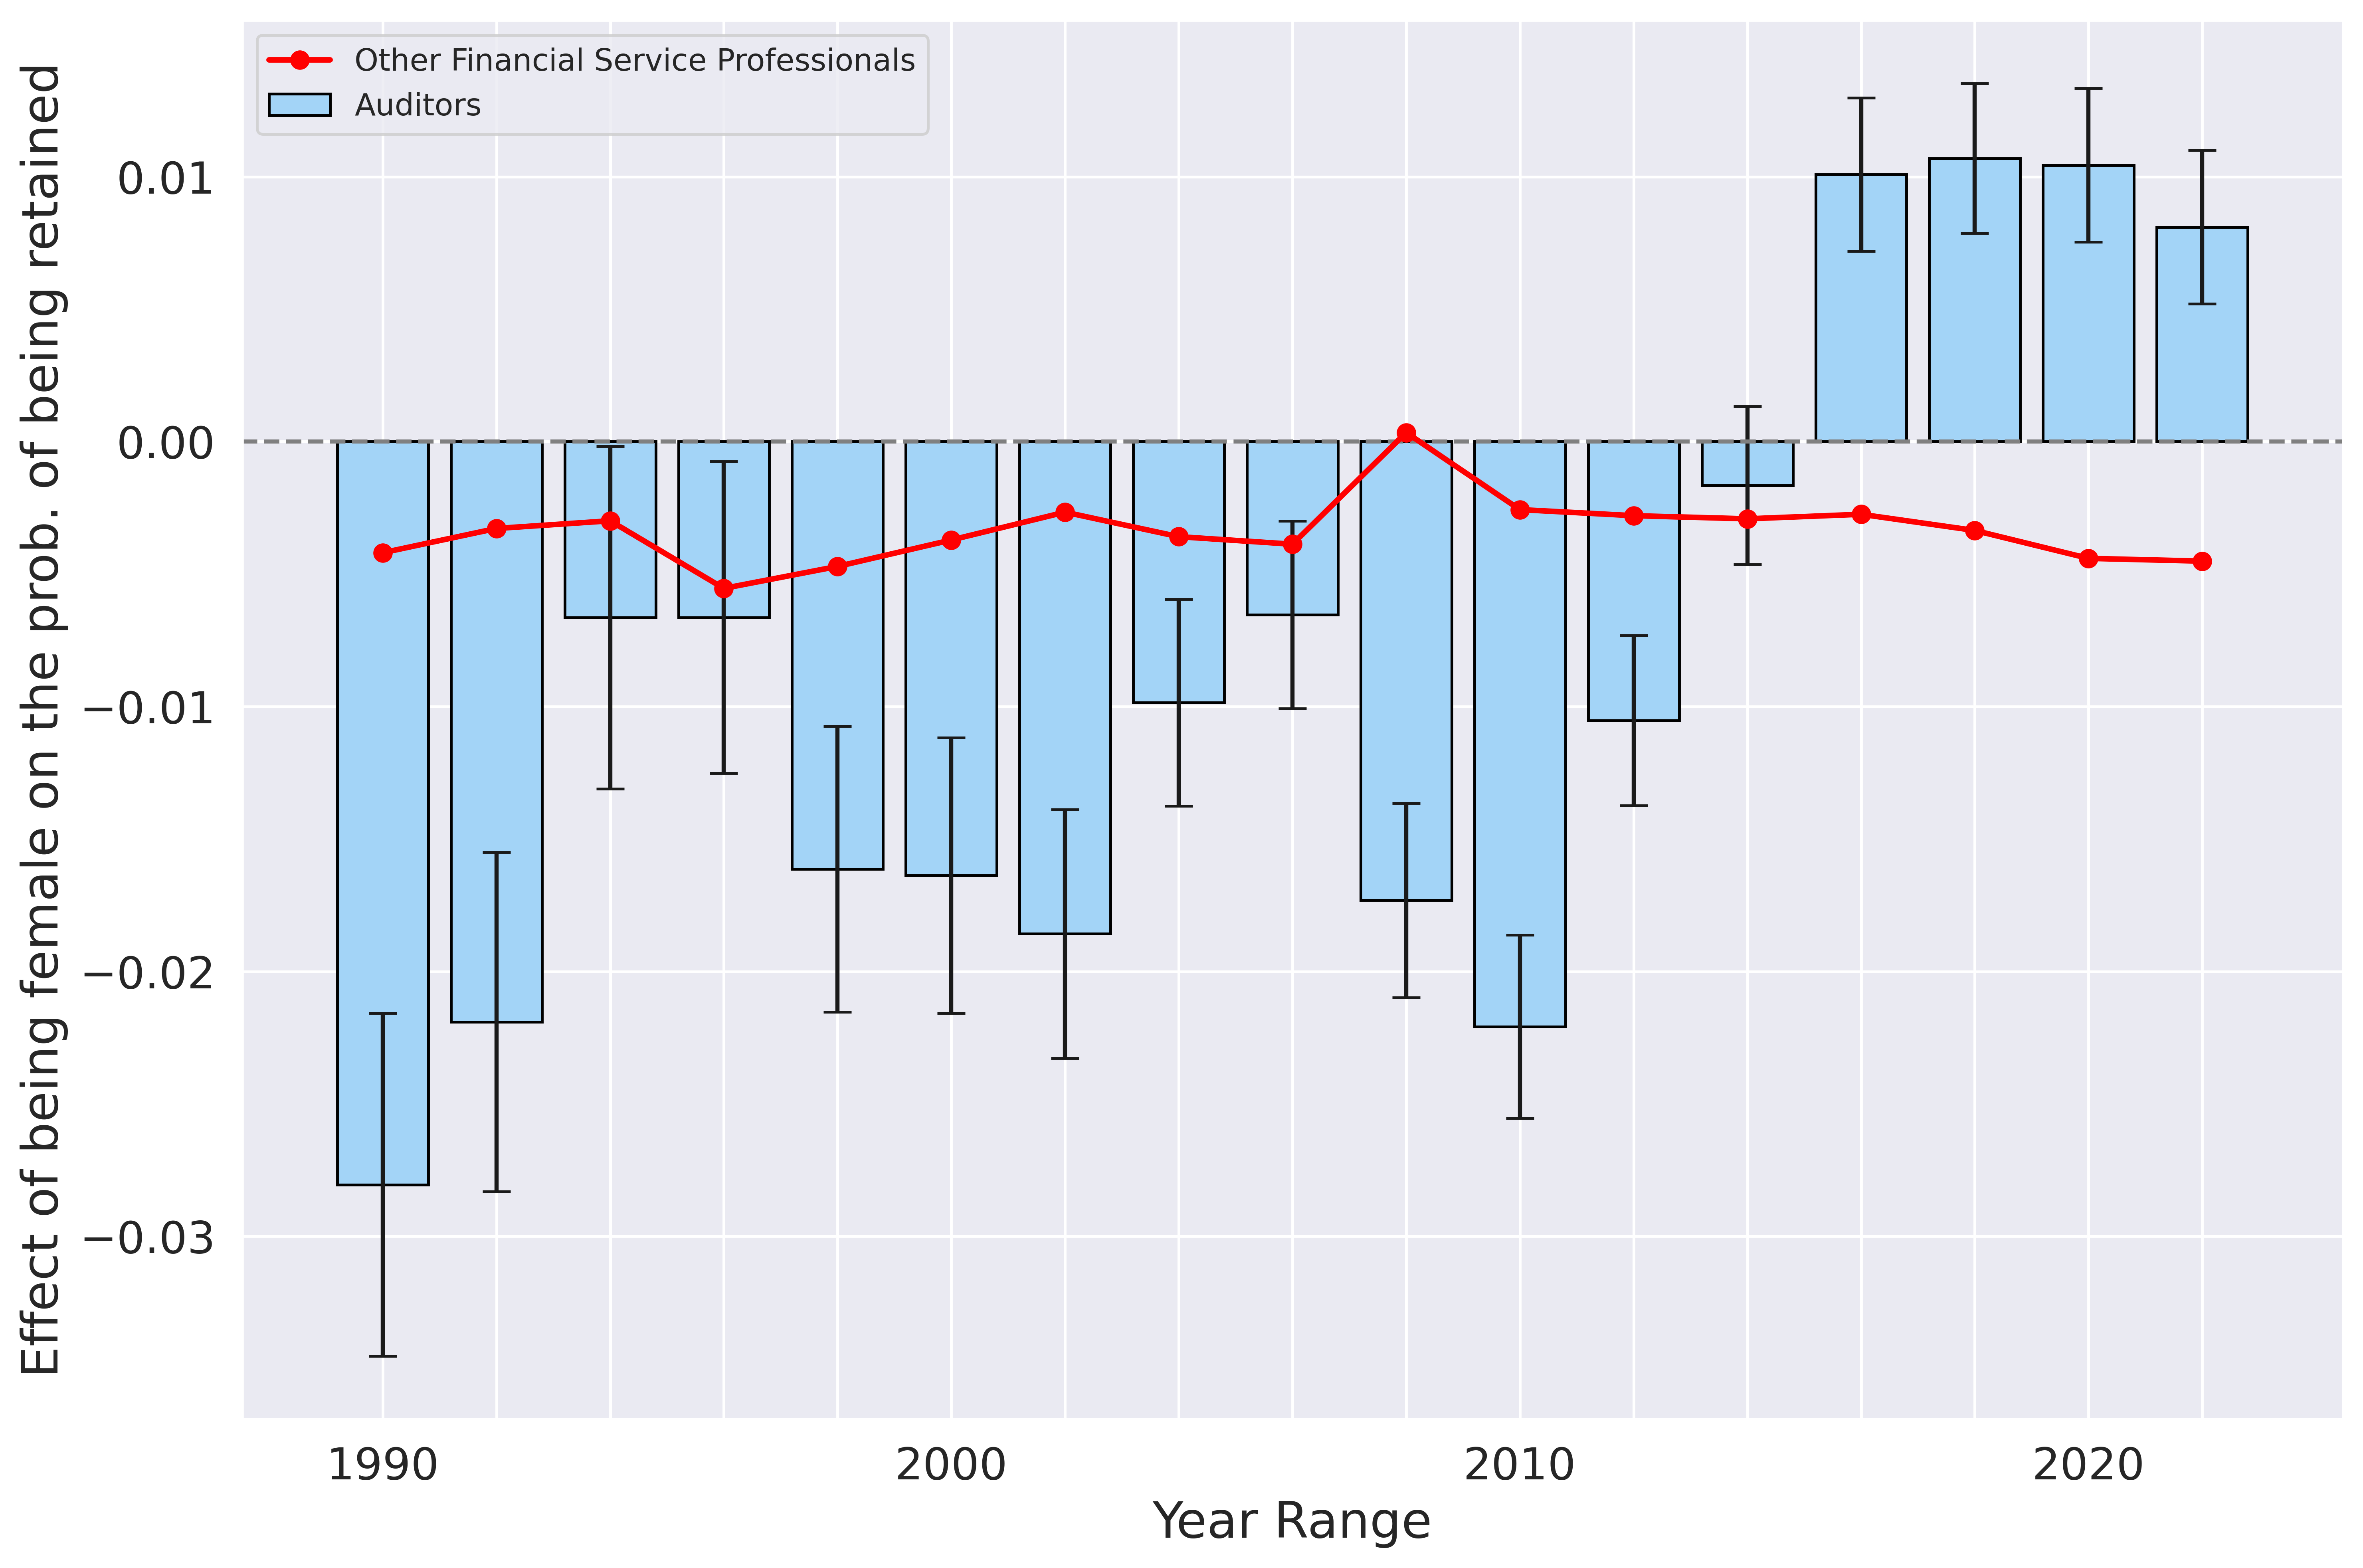
\includegraphics[width=.99\linewidth]{Figures/femaleCoeffPlot.png}
    \label{figure:coeffPlot}
    \footnotesize
    \floatfoot{\textbf{Note}: This figure plots the coefficients and standard error bars from estimating \ref{eq:primaryModel} after expanding it to include additional indicator variables for each two-year period going back to 1990. We also include separate indicator variables for two-year periods in the post-2019 period.}
\end{figure}

%----- Survival Curves -----%
\clearpage
\raggedright
\begin{figure}[t]
    \raggedright
    \captionsetup{labelfont=bf, singlelinecheck=off, justification=raggedright, labelsep=none}
    \caption{: Survival curves}
    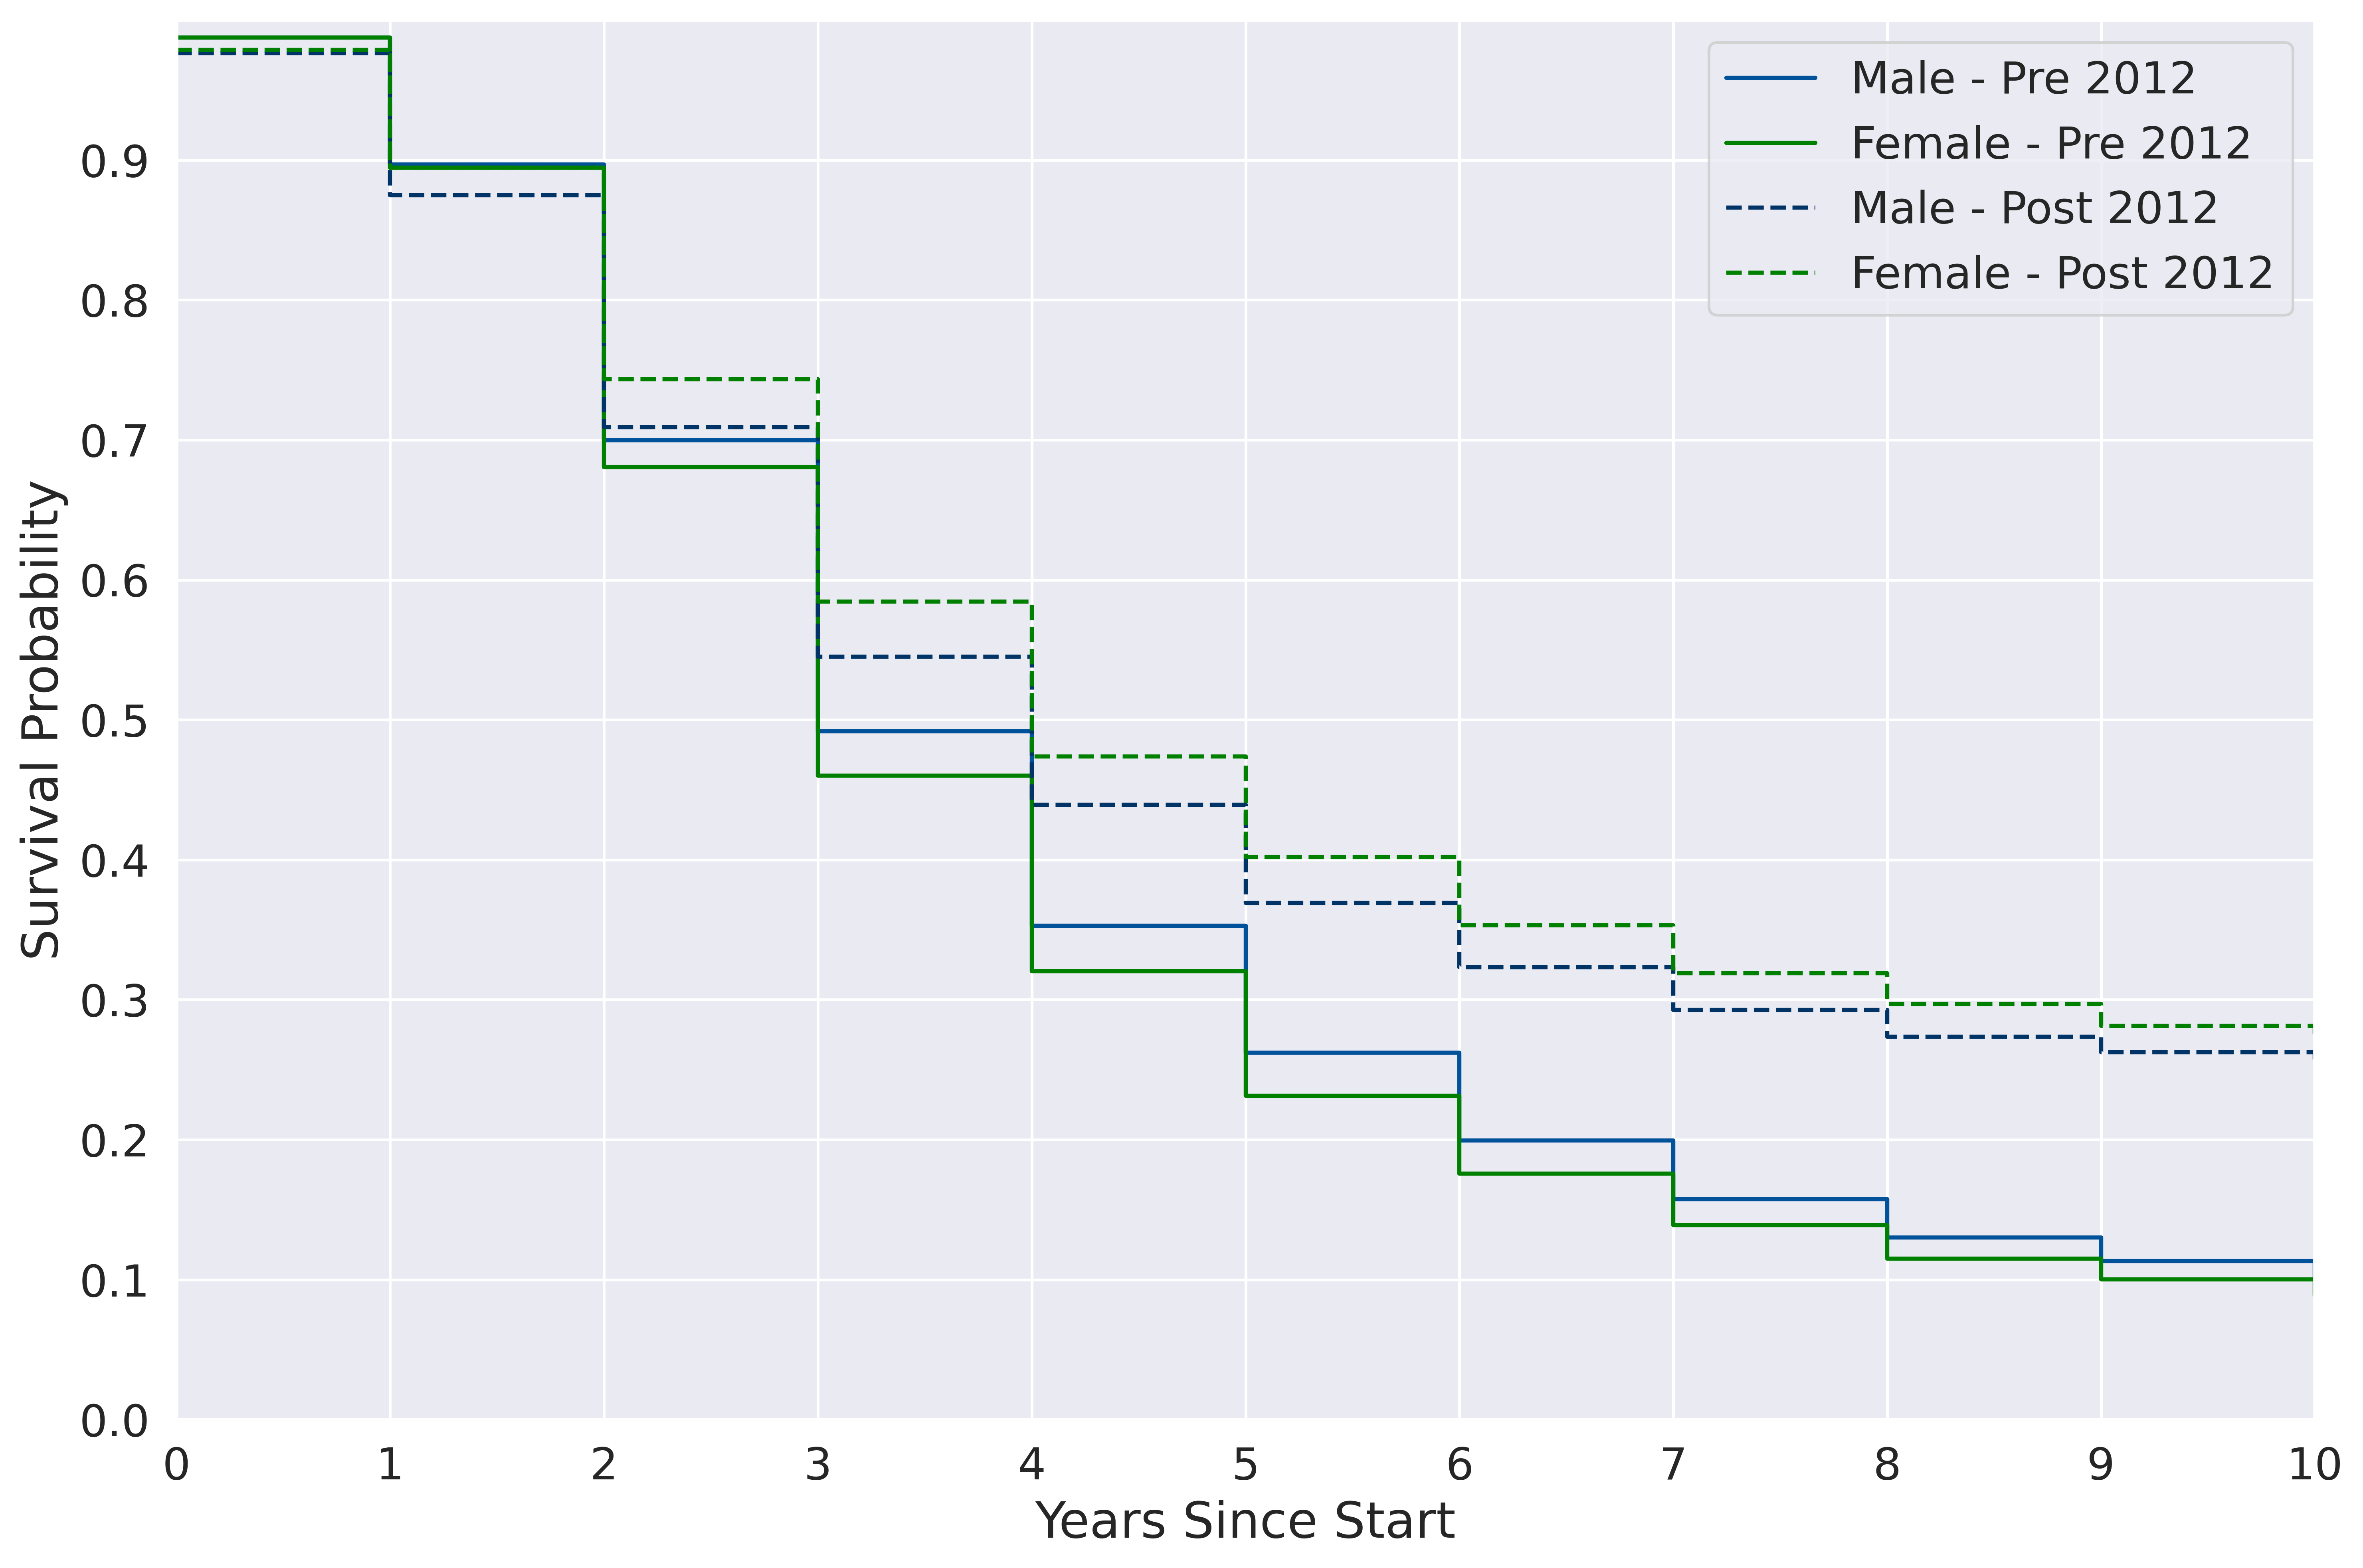
\includegraphics[width=.99\linewidth]{Figures/survivalCurves.png}
    \label{figure:survivalCurves}
    \footnotesize
    \floatfoot{\textbf{Note}: This figure plots separate Kaplan-Meier survival curves for male (in blue) and female (in green) auditors in the pre-2012 (solid lines) and 2012-2023 (dashed lines) periods. }
\end{figure}

%----- Sample Design Table -----%
\clearpage

\clearpage
\begin{landscape}
\begin{table}[!htbp] 
    
    \begin{threeparttable}[b]    
        
        \captionsetup{labelfont=bf, singlelinecheck=off, justification=raggedright, labelsep=none}
        \caption{: Sample design}

        \raggedright
        \hspace*{-\leftmargin}
    
        \normalsize
        \begin{tabular}{ l c c c}\\[-1.8ex]\hline \hline \\[-1.8ex]\underline{Auditor sample}& \underline{Unique employees} & \underline{Unique positions} & \underline{Employee-years} \\Auditors associated with Big 4 firms in Revelio data & 192,245 & 292,897 & \\ \quad Less positions with missing or invalid start/end dates &(2,478) & (3,890) & \\ \quad Less auditors that move between B4 firms &(5,258) & (13,652) & \\ \quad Less auditors missing educational data &(18,125) & (24,495) & \\ \quad Less internship positions &\underline{(19,127)} & (47,488) & \\ Exploded to create auditor-year sample &147,257 &  & 766,730\\ \quad Less auditor-years after 2023 &\underline{(1,684)} & & \underline{(53,116)}\\ Primary sample &145,573& &713,614\\ \quad Less observations without reliable ranks &\underline{(75,057)} & & \underline{(428,615)}\\ Sample for rank and promotion analysis &70,516 &  & 284,999\\\\ \underline{Other financial services sample} & & &\\Employees in finanical services positions comparable to auditing & 4,289,903 & 7,682,481 & \\ \quad Less positions with missing or invalid start/end dates &(490,118) & (587,445) & \\ \quad Less excluded companies (e.g., self-employed, H\&R Block, no company ID) &(496,465) & (1,105,800) & \\ \quad Less employees missing educational data &(741,695) & (1,094,455) & \\ \quad Less internship positions &\underline{(123,075)} & (320,476) & \\ Exploded to create employee-year sample &2,438,550 &  & 23,334,598\\ \quad Less employee-years after 2023 &\underline{(40,631)} & & \underline{(2,208,555)}\\ Primary sample &2,397,919& &21,126,043\\\\[-1.8ex]\hline \hline \\[-1.8ex]\end{tabular}
        
        \begin{tablenotes}
            \footnotesize
            \item \textbf{Note}: This table describes the screening process used to produce the sample used in our primary analysis.   
        \end{tablenotes}
        \label{table:sampleDesign}
    \end{threeparttable}
\end{table}
\end{landscape}

%----- Summary Statistics ----%
\clearpage
\begin{table}[!htbp] 
    
    \begin{threeparttable}[b]    
        
        \captionsetup{labelfont=bf, singlelinecheck=off, justification=raggedright, labelsep=none}
        \caption{: Gender differences in mean values}

        \raggedright
        \hspace*{-\leftmargin}


        \small

        Panel A: Auditor sample
        \begin{tabular}{lcccc}\\[-1.8ex]\hline \hline \\[-1.8ex]
                    &\hspace{1.2mm} Total (N =      713,614) \hspace{1.1mm}&\hspace{1.2mm} Female (N =      311,616) \hspace{1.1mm}&\hspace{1.2mm} Male (N =      401,998) \hspace{1.1mm}& \hspace{1.1mm} Difference  \hspace{1.1mm}\\
                    &     mean/sd&     mean/sd&     mean/sd&           p\\
\midrule
\RETAINED            &       0.832&       0.830&       0.834&       0.000\\
                    &     (0.374)&     (0.375)&     (0.372)&            \\
\PROMOTED               &       0.127&       0.128&       0.126&       0.146\\
                    &     (0.333)&     (0.334)&     (0.332)&            \\
\TOPUNIVERSITY      &       0.159&       0.148&       0.168&       0.000\\
                    &     (0.366)&     (0.355)&     (0.374)&            \\
\MASTERS      &       0.475&       0.469&       0.480&       0.000\\
                    &     (0.499)&     (0.499)&     (0.500)&            \\
\APIRACE                 &       0.103&       0.107&       0.099&       0.000\\
                    &     (0.304)&     (0.309)&     (0.299)&            \\
\BLACKRACE               &       0.081&       0.089&       0.076&       0.000\\
                    &     (0.273)&     (0.285)&     (0.264)&            \\
\OTHERRACE               &       0.066&       0.070&       0.062&       0.000\\
                    &     (0.248)&     (0.256)&     (0.242)&            \\
\\[-1.8ex]\hline \hline \\[-1.8ex] \end{tabular}

        Panel B: Other financial services sample
        \begin{tabular}{lcccc}\\[-1.8ex]\hline \hline \\[-1.8ex]
                    &Total (N =   21,126,043)&Female (N =    7,233,035)&Male (N =   13,893,008)&  Difference\\
                    &     mean/sd&     mean/sd&     mean/sd&           p\\
\midrule
\RETAINED            &       0.910&       0.909&       0.911&       0.000\\
                    &     (0.286)&     (0.288)&     (0.284)&            \\
\TOPUNIVERSITY      &       0.187&       0.172&       0.194&       0.000\\
                    &     (0.390)&     (0.378)&     (0.395)&            \\
\MASTERS      &       0.401&       0.368&       0.418&       0.000\\
                    &     (0.490)&     (0.482)&     (0.493)&            \\
\APIRACE                 &       0.070&       0.075&       0.067&       0.000\\
                    &     (0.255)&     (0.263)&     (0.251)&            \\
\BLACKRACE               &       0.072&       0.087&       0.064&       0.000\\
                    &     (0.258)&     (0.281)&     (0.245)&            \\
\OTHERRACE               &       0.056&       0.063&       0.052&       0.000\\
                    &     (0.229)&     (0.243)&     (0.221)&            \\
\\[-1.8ex]\hline \hline \\[-1.8ex] \end{tabular}
        
        \begin{tablenotes}
            \footnotesize
            \item \textbf{Note}: This table presents sample means for the variables used in our analysis, both for the pooled sample and separately for male and female financial service professionals. The statistical significance of differences in means between male and female professionals is indicated by p-values in the last column. Variable definitions are provided in Appendix \ref{appendix:variableDefinitions}.   
        \end{tablenotes}
        \label{table:summaryStats}
    \end{threeparttable}
\end{table}

%----- Retention for auditors vs other financial services -----%
\clearpage
%\begin{landscape}
\begin{table}[!htbp]
    \begin{threeparttable}[b]
        
        \captionsetup{labelfont=bf, singlelinecheck=off, justification=raggedright, labelsep=none}
        \caption{: Changes in female retention - auditing vs other financial services}  
        
        \raggedright
        \hspace*{-\leftmargin}
        \vspace*{-0.75cm}
        \small

        \noindent
        {
\def\sym#1{\ifmmode^{#1}\else\(^{#1}\)\fi}
\begin{tabular}{l*{4}{D{.}{.}{-1}}}
\\[-1.8ex]\hline \hline \\[-1.8ex]
                    &\multicolumn{1}{c}{(1)}&\multicolumn{1}{c}{(2)}&\multicolumn{1}{c}{(3)}&\multicolumn{1}{c}{(4)}\\
                    &\multicolumn{1}{c}{\shortstack{Auditors\\ DV = Retained}}&\multicolumn{1}{c}{\shortstack{Other Financial Svc.\\ DV = Retained}}&\multicolumn{1}{c}{\shortstack{Investment Bankers\\ DV = Retained}}&\multicolumn{1}{c}{\shortstack{Credit Analysts\\ DV = Retained}}\\
\midrule
\FEMALExPREX     &      -0.012\sym{***}&      -0.003\sym{***}&      -0.021\sym{***}&       0.007\sym{***}\\
                    &     (0.001)         &     (0.000)         &     (0.002)         &     (0.001)         \\
\FEMALExXtoXI    &      -0.022\sym{***}&      -0.003\sym{***}&      -0.025\sym{***}&       0.010\sym{***}\\
                    &     (0.003)         &     (0.001)         &     (0.006)         &     (0.003)         \\
\FEMALExXIItoXIII    &      -0.011\sym{***}&      -0.003\sym{***}&      -0.016\sym{***}&       0.008\sym{***}\\
                    &     (0.003)         &     (0.001)         &     (0.006)         &     (0.003)         \\
\FEMALExXIVtoXV    &      -0.002         &      -0.003\sym{***}&      -0.031\sym{***}&       0.013\sym{***}\\
                    &     (0.003)         &     (0.000)         &     (0.005)         &     (0.003)         \\
\FEMALExXVItoXVII    &       0.010\sym{***}&      -0.003\sym{***}&      -0.026\sym{***}&       0.008\sym{***}\\
                    &     (0.003)         &     (0.000)         &     (0.005)         &     (0.002)         \\
\FEMALExXVIIItoXIX    &       0.011\sym{***}&      -0.003\sym{***}&      -0.017\sym{***}&       0.006\sym{***}\\
                    &     (0.003)         &     (0.000)         &     (0.004)         &     (0.002)         \\
\FEMALExPOSTXIX    &       0.009\sym{***}&      -0.004\sym{***}&      -0.019\sym{***}&       0.011\sym{***}\\
                    &     (0.002)         &     (0.000)         &     (0.003)         &     (0.002)         \\
\MASTERS      &      -0.018\sym{***}&      -0.004\sym{***}&      -0.005\sym{***}&      -0.012\sym{***}\\
                    &     (0.001)         &     (0.000)         &     (0.001)         &     (0.001)         \\
\TOPUNIVERSITY      &      -0.001         &      -0.006\sym{***}&      -0.018\sym{***}&      -0.004\sym{***}\\
                    &     (0.001)         &     (0.000)         &     (0.001)         &     (0.001)         \\
\APIRACE                 &      -0.006\sym{***}&      -0.006\sym{***}&      -0.016\sym{***}&      -0.003         \\
                    &     (0.001)         &     (0.000)         &     (0.002)         &     (0.002)         \\
\BLACKRACE               &       0.001         &      -0.005\sym{***}&      -0.011\sym{***}&      -0.002         \\
                    &     (0.002)         &     (0.000)         &     (0.002)         &     (0.001)         \\
\OTHERRACE               &      -0.004\sym{**} &      -0.007\sym{***}&      -0.003         &      -0.000         \\
                    &     (0.002)         &     (0.000)         &     (0.003)         &     (0.002)         \\
Constant            &       0.843\sym{***}&       0.916\sym{***}&       0.881\sym{***}&       0.882\sym{***}\\
                    &     (0.001)         &     (0.000)         &     (0.001)         &     (0.001)         \\
\midrule
Observations        &     713,607         &  21,083,773         &     406,761         &     898,003         \\
Adjusted R-squared  &       0.005         &       0.031         &       0.053         &       0.024         \\
Fixed effects       &       C,Y,E         &       C,Y,E         &       C,Y,E         &       C,Y,E         \\
\\[-1.8ex]\hline \hline \\[-1.8ex]
\end{tabular}
}

        
        \begin{tablenotes}
            \footnotesize
            \item \textbf{Note}: This table presents the results of estimating \ref{eq:primaryModel} to model employee retention. Column 1 uses a sample of auditors, Column 2 uses a broad sample of non-auditing financial service positions, Column 3 uses a sample investment bankers, and Column 4 uses a sample of credit analysts. Robust standard errors clustered by employee are presented in parentheses. Fixed effects for each model are indicated using the following symbols: C = cohort-year, Y = calendar-year, E = employer. Sample sizes may differ from those shown in Table \ref{table:sampleDesign} due to dropped singleton observations or missing values for some variables. The symbols *, **, and *** indicate p-values of \textless\, .10, \textless\, .05, and \textless\, .01 respectively. Variable definitions are provided in Appendix \ref{appendix:variableDefinitions}. 
        \end{tablenotes}
        \label{table:interactionModels}
    \end{threeparttable}
\end{table}
%\end{landscape}

%----- Robustness specifications -----%
\clearpage
\begin{table}[!htbp]
    \begin{threeparttable}[b]
        
        \captionsetup{labelfont=bf, singlelinecheck=off, justification=raggedright, labelsep=none}
        \caption{: Robustness tests}  
        
        \raggedright
        \hspace*{-\leftmargin}
        \vspace*{-0.75cm}
        \normalsize

        \noindent
        {
\def\sym#1{\ifmmode^{#1}\else\(^{#1}\)\fi}
\begin{tabular}{l*{2}{D{.}{.}{-1}}}
\\[-1.8ex]\hline \hline \\[-1.8ex]
                    &\multicolumn{1}{c}{(1)}&\multicolumn{1}{c}{(2)}\\
                    &\multicolumn{1}{c}{\shortstack{Auditors\\ DV = Hazard}}&\multicolumn{1}{c}{\shortstack{Auditors\\ DV = Retained}}\\
\midrule
\FEMALExPREX     &       0.062\sym{***}&      -0.011\sym{***}\\
                    &     (0.008)         &     (0.001)         \\
\FEMALExXtoXI    &       0.077\sym{***}&      -0.023\sym{***}\\
                    &     (0.020)         &     (0.004)         \\
\FEMALExXIItoXIII    &       0.007         &      -0.010\sym{***}\\
                    &     (0.019)         &     (0.003)         \\
\FEMALExXIVtoXV    &      -0.047\sym{***}&      -0.001         \\
                    &     (0.018)         &     (0.003)         \\
\FEMALExXVItoXVII    &      -0.094\sym{***}&       0.010\sym{***}\\
                    &     (0.017)         &     (0.003)         \\
\FEMALExXVIIItoXIX    &      -0.097\sym{***}&       0.012\sym{***}\\
                    &     (0.017)         &     (0.003)         \\
\FEMALExPOSTXIX    &      -0.094\sym{***}&       0.009\sym{***}\\
                    &     (0.013)         &     (0.002)         \\
Constant            &                     &       0.843\sym{***}\\
                    &                     &     (0.001)         \\
\midrule
Observations        &     713,614         &     696,009         \\
Adjusted R-squared  &                     &       0.007         \\
Fixed effects       &         Y,E         &     C,E,Y*M         \\
\\[-1.8ex]\hline \hline \\[-1.8ex]
\end{tabular}
}

        
        \begin{tablenotes}
            \footnotesize
            \item \textbf{Note}: This table presents the results of two robustness tests. Column 1 presents a Cox proportional hazard model estimation instead of the OLS approach used in our primary results. Column 2 adds metropolitan area-by-year fixed effects to our OLS model. Control variables from Table \ref{table:interactionModels} are included in all columns, but their coefficients are not tabulated for parsimony. Robust standard errors clustered by employee are presented in parentheses. Fixed effects for each model are indicated using the following symbols: C = cohort-year, Y = calendar-year, E = employer, Y-M = year-by-metropolitan area. Sample sizes may differ from those shown in Table \ref{table:sampleDesign} due to dropped singleton observations or missing values for some variables. The symbols *, **, and *** indicate p-values of \textless\, .10, \textless\, .05, and \textless\, .01 respectively. Variable definitions are provided in Appendix \ref{appendix:variableDefinitions}.  
        \end{tablenotes}
        \label{table:robustnessModels}
    \end{threeparttable}
\end{table}

%----- Promotion analysis -----%
\clearpage
\begin{table}[!htbp]
    \begin{threeparttable}[b]
        
        \captionsetup{labelfont=bf, singlelinecheck=off, justification=raggedright, labelsep=none}
        \caption{: Promotion analysis}  
        
        \raggedright
        \hspace*{-\leftmargin}
        \vspace*{-0.75cm}
        \normalsize

        \noindent
        {
\def\sym#1{\ifmmode^{#1}\else\(^{#1}\)\fi}
\begin{tabular}{l*{1}{D{.}{.}{-1}}}
\\[-1.8ex]\hline \hline \\[-1.8ex]
                    &\multicolumn{1}{c}{(1)}\\
                    &\multicolumn{1}{c}{\shortstack{Retained\\Auditors < Partner\\ DV = Promoted}}\\
\midrule
\FEMALExPREX     &      -0.007\sym{***}\\
                    &     (0.002)         \\
\FEMALExXtoXI    &      -0.011\sym{*}  \\
                    &     (0.006)         \\
\FEMALExXIItoXIII    &      -0.001         \\
                    &     (0.005)         \\
\FEMALExXIVtoXV    &      -0.001         \\
                    &     (0.004)         \\
\FEMALExXVItoXVII    &       0.004         \\
                    &     (0.004)         \\
\FEMALExXVIIItoXIX    &       0.010\sym{***}\\
                    &     (0.004)         \\
\FEMALExPOSTXIX    &       0.008\sym{***}\\
                    &     (0.002)         \\
Constant            &       0.158\sym{***}\\
                    &     (0.001)         \\
\midrule
Observations \quad \quad \quad \quad \quad \quad \quad \quad \quad \quad \quad \quad &     229,083         \\
Adjusted R-squared  &       0.033         \\
Fixed effects       &       C,Y,E         \\
\\[-1.8ex]\hline \hline \\[-1.8ex]
\end{tabular}
}

        
        \begin{tablenotes}
            \footnotesize
            \item \textbf{Note}: This table presents the results of a promotion analysis by replacing the dependent variable in \ref{eq:primaryModel} with \textit{Promoted} instead of \textit{Retained}. Control variables from Table \ref{table:interactionModels} are included in all columns, but their coefficients are not tabulated for parsimony. Robust standard errors clustered by employee are presented in parentheses. Fixed effects for each model are indicated using the following symbols: C = cohort-year, Y = calendar-year, E = employer. Sample sizes may differ from those shown in Table \ref{table:sampleDesign} due to dropped singleton observations or missing values for some variables. The symbols *, **, and *** indicate p-values of \textless\, .10, \textless\, .05, and \textless\, .01 respectively. Variable definitions are provided in Appendix \ref{appendix:variableDefinitions}.  
        \end{tablenotes}
        \label{table:promotionModels}
    \end{threeparttable}
\end{table}

%----- Equalized leave -----%
\clearpage
\begin{table}[!htbp]
    \begin{threeparttable}[b]
        
        \captionsetup{labelfont=bf, singlelinecheck=off, justification=raggedright, labelsep=none}
        \caption{: Equalized family leave}  
        
        \raggedright
        \hspace*{-\leftmargin}
        \vspace*{-0.75cm}
        \normalsize
        
        \noindent
        {
\def\sym#1{\ifmmode^{#1}\else\(^{#1}\)\fi}
\begin{tabular}{l*{2}{D{.}{.}{-1}}}
\\[-1.8ex]\hline \hline \\[-1.8ex]
                    &\multicolumn{1}{c}{(1)}&\multicolumn{1}{c}{(2)}\\
                    &\multicolumn{1}{c}{\shortstack{Auditors\\ DV = Retained}}&\multicolumn{1}{c}{\shortstack{Retained\\Auditors < Partner\\ DV = Promoted}}\\
\midrule
\FEMALE              &      -0.009\sym{***}&      -0.003         \\
                    &     (0.001)         &     (0.002)         \\
\FEMALExPREEQTHREE     &      -0.006         &      -0.002         \\
                    &     (0.005)         &     (0.010)         \\
\FEMALExPREEQTWO     &       0.008         &      -0.007         \\
                    &     (0.005)         &     (0.009)         \\
\FEMALExPREEQONE     &       0.008         &       0.008         \\
                    &     (0.005)         &     (0.008)         \\
\FEMALExPOSTEQ      &       0.017\sym{***}&       0.011\sym{***}\\
                    &     (0.002)         &     (0.003)         \\
\POSTEQ             &      -0.026\sym{***}&      -0.007\sym{*}  \\
                    &     (0.002)         &     (0.003)         \\
Constant            &       0.852\sym{***}&       0.163\sym{***}\\
                    &     (0.001)         &     (0.002)         \\
\midrule
{Observations}      &     713,607         &     229,083         \\
{Adjusted R-squared}&       0.005         &       0.033         \\
{Fixed effects}     &       C,Y,E         &       C,Y,E         \\
\\[-1.8ex]\hline \hline \\[-1.8ex]
\end{tabular}
}

        
        \begin{tablenotes}
            \footnotesize
            \item \textbf{Note}: This table presents the results of estimating \ref{eq:equalleave}. Column 1 (2) uses \RETAINED\ (\PROMOTED) as the dependent variable. Robust standard errors clustered by employee are presented in parentheses. Control variables and stand-alone pre-period indicators are included, but their coefficients are not tabulated for parsimony. Fixed effects for each model are indicated using the following symbols: C = cohort-year, Y = calendar-year, E = employer. Sample sizes may differ from those shown in Table \ref{table:sampleDesign} due to dropped singleton observations or missing values for some variables. The symbols *, **, and *** indicate p-values of \textless\, .10, \textless\, .05, and \textless\, .01 respectively. Variable definitions are provided in Appendix \ref{appendix:variableDefinitions}. 
        \end{tablenotes}
        \label{table:eqFamModels}
    \end{threeparttable}
\end{table}


%--------------------%
%----- Appendix -----%
%--------------------%

\appendix

\renewcommand{\tablename}{Table} 
\renewcommand{\thetable}{A\arabic{table}} 
\setcounter{table}{0}

\clearpage
\Large
Appendix
\small

\singlespacing

\begin{table}[h!]
    \centering
    \caption{Roles used in initial Revelio query}
    
\centering
\begin{tabular}{p{7cm}p{7cm}}
\toprule
Column 1 & Column 2 \\
\midrule
actuarial & financial planning analysis \\
actuarial analyst & financial planning analyst \\
actuary & financial reporting \\
aml analyst & financial reporting analyst \\
audit & fraud analyst \\
auditor & fraud investigator \\
banking consultant & investment analyst \\
broker & investment banking \\
brokerage & investment banking analyst \\
business controller & investment consultant \\
capital markets & investments \\
cfo & mergers acquisitions \\
commercial finance & portfolio analyst \\
commercial underwriter & pricing analyst \\
controller & project controller \\
credit analyst & quantitative analyst \\
equity analyst & sap fico consultant \\
equity research & stock controller \\
equity research analyst & tax \\
finance controller & tax accountant \\
financial adviser & tax analyst \\
financial analyst fp a & tax consultant \\
financial consultant & trade finance \\
financial controller & trader \\
financial officer & trading \\
financial planner & underwriter \\
financial planning & underwriting \\

\bottomrule
\end{tabular}

    \label{table:rolesTable}
\end{table}

\clearpage
\begin{table}[h!]
    \centering
    \caption{\\The top 50 companies by employee count in the other financial services sample}
    
\centering
\begin{tabular}{p{7cm}p{7cm}}
\toprule
Column 1 & Column 2 \\
\midrule
JPMorgan Chase & Northwestern Mutual \\
Bank of America & AIG \\
Wells Fargo & GE Capital \\
Morgan Stanley & Internal Revenue Service \\
Merrill Lynch & Travelers \\
Citi & MetLife \\
Goldman Sachs & Liberty Mutual Insurance \\
Fidelity Investments & Aon \\
UBS & CBRE \\
Credit Suisse & Raymond James \\
Deutsche Bank & HSBC \\
Charles Schwab & BDO USA, LLP \\
Prudential Financial & New York Life Insurance Company \\
RSM US LLP & Primerica \\
BNY Mellon & IBM \\
Edward Jones & Coldwell Banker Residential Brokerage \\
BlackRock & RBC Capital Markets \\
U.S. Bank & Barclays Investment Bank \\
PNC & The Hartford \\
Capital One & American Express \\
State Street & AT\&T \\
Lehman Brothers & JLL \\
Arthur Andersen & CLA (CliftonLarsonAllen) \\
Vanguard & TD Ameritrade \\
Ameriprise Financial Services, LLC & Accenture \\

\bottomrule
\end{tabular}

    \label{table:employerTable}
\end{table}

\clearpage
\centering
\begin{longtable}{>{\raggedright\arraybackslash}p{3cm}p{13cm}}

%----- Header/Footer Setup -----%
%\captionsetup{labelfont=bf, singlelinecheck=off, justification=raggedright, labelsep=none}
\caption{Variable definitions}

\\[-1.8ex]\hline \hline \\[-1.8ex]
\endfirsthead

\multicolumn{2}{l}%
{{\textit{Continued from previous page}}} \\
\midrule
\endhead

\multicolumn{2}{r}{{\textit{Continued on next page}}}
\endfoot

\multicolumn{2}{r}{{ }}
\endlastfoot

%----- Variable Definitions -----%

\RETAINED & An indicator variable set equal to 1 if the professional remains with the firm the following year, 0 otherwise. \\
\midrule

\PROMOTED & An indicator variable set equal to 1 if the auditor is promoted to a higher rank in the following year, 0 otherwise. \\
\midrule

\FEMALE & An indicator variable set equal to 1 if the professional is classified as female by the \textit{sex\_predicted} field Revelio, and 0 otherwise. \\
\midrule

\MASTERS & An indicator variable set equal to 1 if the auditor holds a master's degree or higher, and 0 otherwise, according to the \textit{highest\_dgree} field in the Revelio data \\
\midrule

\TOPUNIV & An indicator variable set equal to 1 if the professional attended a top university as defined by \textcite{FGH2022}.\\
\midrule

\APIRACE & An indicator variable set equal to 1 if the professional is classified as API (i.e., Asian and Pacific Islander) by the \textit{ethnicity\_predicted} field in Revelio, 0 otherwise.\\
\midrule

\BLACKRACE & An indicator variable set equal to 1 if the professional is classified as Black by the \textit{ethnicity\_predicted} field in Revelio, 0 otherwise.\\
\midrule

\OTHERRACE & An indicator variable set equal to 1 if the professional is classified as any ethnicity other than API, Black, or White by the \textit{ethnicity\_predicted} field in Revelio, 0 otherwise.\\

\\[-1.8ex]\hline \hline \\[-1.8ex]

\label{appendix:variableDefinitions}
\end{longtable}


 
\label{table:variableDefinitions} 



\end{document}


